\chapter{The Standard Model}

\textit{"...it turns out that based on their findings, which will be confirmed
or contradicted when the Swiss machine is up and running, turns out there's
slightly more positive than negative muons in all of our atoms, which would
justify the faith of all the believers of the world, make you more
optimistic, and give us an explanation for how we might have all come to this
moment from the primordial slime."}
\vspace{5mm}
\begin{flushright}
--- Bill Clinton, Davos 2011
\end{flushright}

\newpage
\noindent
Our current best understanding of Nature is that the dynamics of matter is governed
by four fundamental forces. General Relativity (GR) provides a
description of spacetime, the arena in which matter exists and interacts, and asserts
that spacetime is not a static entity but is rather dynamically shaped by the presence
of matter. It also explains one of the forces, the gravitational force, as an apparent
phenomenon arising from geodesic motion in curved spacetime. The Standard Model
(SM) not only describes the remaining three forces, the electromagnetic (EM) force,
the weak force, and the strong force, but also provides a description of matter, and 
elucidates the origin of mass.

The Standard Model is expressed in the language of Quantum Field Theory (QFT). QFT 
extends the domain of quantum mechanics, which characterises the very small, to
the domain of special relativity, which governs the very fast. It does so by
proposing that the fundamental objects are not particles, but rather fields, the
excitations of which are interpreted as particles.

Similarly to classical field theory the system under consideration is characterised
by a Lagrangian density, usually simply called the Lagrangian. According to
the principle of least action, the equations of motion for a system are then derived
by solving the Euler-Lagrange equation \cite{Thomson:2013zua},
\begin{equation}
\partial_\mu \left(\frac{\partial \mathcal{L}}{\partial(\partial_\mu \phi_i)}\right)
- \frac{\partial{\mathcal{L}}}{\partial \phi_i} = 0,
\end{equation}
where $\mathcal{L}$ is the Lagrangian, $\phi_i$ are the fields, partial derivatives
are taken w.r.t. the spacetime coordinates, and Einstein summation convention implies
the sum over repeated indices. The Lagrangian therefore contains all
information about the dynamical system. 

The Lagrangian must be invariant under the transformations which leave the
system it describes physically unchanged. Apart from the Poincar\'e symmetries, which
ensure the physics is invariant w.r.t. translations, rotations, and changes of inertial
reference frame, the defining symmetry of the Standard Model is the internal
$SU(3)_C \times SU(2)_L \times U(1)_Y$ local gauge symmetry.

$SU(3)_C$ group symmetry, where $C$ stands for colour, defines quantum chromodynamics
(QCD), the theory of strong force interactions between quarks and gluons. The electroweak
interactions, a unified theory of the electromagnetic and weak forces, are described by
the $SU(2)_L \times U(1)_Y$ group symmetry. Here, the $L$ refers to left-handed particles
chirality, which is related to the relative direction of particle momentum and spin, and
$Y$ is the weak hypercharge, related to the electric charge and third component of the
weak isospin \cite{Thomson:2013zua}.

The requirement for the Lagrangian to be locally gauge invariant places some constraints
on the allowed terms. Notably, the four-derivative $\partial_\mu$ is replaced by a 
covariant derivative, which introduces the interactions between the matter and gauge
fields. On the other hand, local gauge invariance prohibits the naive mass terms for
both the gauge bosons and fermions \cite{Thomson:2013zua}. This is in stark contrast
with the experimental reality: fermions and weak gauge bosons are massive.

This embarrasing discrepancy is resolved by the Higgs mechanism, which generates the
masses of the fermions and gauge bosons by interactions to the non-zero Higgs field
value at the minimum of the Higgs potential.

\section{Elementary particles}

The particle content of the Standard Model can be classified according to spin, the
intrinsic angular momentum. Particles with half-integer spin obey Fermi-Dirac statistics
and are called fermions, while particles with integer spin obey Bose-Einstein
statistics and are called bosons.

\begin{table}[h]
\centering
\caption{Fermions of the Standard Model}
\label{tab:the:fermions}
\begin{tabular}{c c ccc ccc}
\toprule
 & & \multicolumn{3}{c}{generation} & \multicolumn{3}{c}{interaction} \\ 
 & & \nth{1} & \nth{2} & \nth{3} & weak & EM & strong \\
\midrule
\multirow{2}{*}{\textbf{Quarks}}
& up-type    & $u$ & $c$ & $t$ & \cmark & \cmark & \cmark \\
& down-type  & ~$d$~ & ~$s$~ & ~$b$~ & \cmark & \cmark & \cmark \\
\multirow{2}{*}{\textbf{Leptons}}
& charged    & ~$e$~ & ~$\mu$~ & ~$\tau$~ & \cmark & \cmark & \\
& neutrinos  & ~$\nu_e$~ & ~$\nu_\mu$~ & ~$\nu_\tau$~ & \cmark & & \\
\bottomrule
\end{tabular}
\end{table}

All known fundamental (i.e. non-composite) fermions have spin-$\frac{1}{2}$ and are
shown in Table \ref{tab:the:fermions}. They are categorised in quarks, which interact via
the strong force, and leptons, which don't. Both quarks and charged leptons interact
via the electromagnetic force, and all fermions interact via the weak force. There
are three generations of up- and down-type quarks as well as charged leptons and
neutrinos. Only the mass differs between generations, other quantum numbers are
identical.

\begin{table}[h]
\centering
\caption{Bosons of the Standard Model}
\label{tab:the:bosons}
\begin{tabular}{c c ccc}
\toprule
 & & & multiplicity & interaction \\ 
\midrule
\multirow{4}{*}{\textbf{Spin-1}}
 & photon    & $\gamma$ & 1 & EM      \\
 & $Z$ boson & $Z$      & 1 & weak    \\
 & $W$ boson & $W^\pm$  & 2 & weak    \\
 & gluon     & $g$      & 8 & strong  \\
\textbf{Spin-0} & Higgs boson & $H$ & 1 &  \\
\bottomrule
\end{tabular}
\end{table}

Spin-1 bosons in the Standard Model are the force carriers, the photon for the
electromagnetic interaction, the $Z$ and $W$ bosons for the weak interaction,
and the gluons for the strong interaction. Photons and gluons are massless, but
the $Z$ and $W$ bosons are one of the heaviest fundamental particles in the
Standard Model.

\section{Electroweak interactions}

A unified theory of quantum electrodynamics (QED) and the weak interaction was developed
by Glashow, Salam, and Weinberg (GSW) in the 1960s \cite{Thomson:2013zua}. 

weak isospin doublet

TODO: introduce $g_Z$

TODO: explain the terms in the covariant derivative

\section{The Higgs mechanism}

In the GSW model, the Higgs model is a weak isospin doublet of complex scalar fields \cite{Thomson:2013zua},
\begin{equation}
\phi = \begin{pmatrix} \phi^+ \\ \phi^0 \end{pmatrix},
\end{equation}
described by the Lagrangian
\begin{equation}
\mathcal{L} = (\partial_\mu \phi)^\dag (\partial^\mu \phi) - \mu^2(\phi^\dag\phi) - \lambda(\phi^\dag \phi)^2,
\label{eq:higgs_lag}
\end{equation}
where the potential $V(x) = \mu^2(\phi^\dag\phi) + \lambda(\phi^\dag \phi)^2$
has an infinite number of minima satisfying $\phi^\dag \phi = -\frac{\mu^2}{2\lambda}$
in the case when $\mu^2 < 0$. The symmetry is spontaneously broken by choosing a
particular minimum from the allowed set, and the fields can be expanded around the chosen minimum.
In the unitary gauge, the Higgs doublet is written as
\begin{equation}
\phi(x) = \frac{1}{\sqrt{2}} \begin{pmatrix} 0 \\ v + h(x) \end{pmatrix},
\end{equation}
where the dependence on $x$ has been made explicit to distinguish the constant
$v$ from the Higgs boson $h(x)$.

In order to make the Lagrangian in Eq. \ref{eq:higgs_lag} invariant under the electroweak
$SU(2)_L \times U(1)_Y$ symmetry, the derivative is replaced by the covariant
derivative \cite{Thomson:2013zua}
\begin{equation}
\partial_\mu \rightarrow D_\mu = \partial_\mu + i g_W \mathbf{T} \cdot \mathbf{W}_\mu
+ i g' \frac{Y}{2} B_\mu.
\end{equation}
The kinetic term in the rewritten Lagrangian, $(D_\mu \phi)^\dag (D^\mu \phi)$, generates the
masses of the gauge bosons. Rearranging, the masses of gauge bosons can be read off as
\begin{equation}
m_W = \frac{1}{2} g_W v,
\end{equation}
\begin{equation}
m_A = 0,
\end{equation}
\begin{equation}
m_Z = \frac{1}{2}v\sqrt{g_W^2 + g'^2}.
\end{equation}
Furthermore, the kinetic term also contains the interaction terms between the gauge bosons
and the Higgs boson $h(x)$. Both the couplings to the $W$, $g_{HWW}=g_W m_W$, and to the $Z$,
$g_{HZZ} = g_Z m_Z$, are proportional to their respective masses \cite{Thomson:2013zua}.

Similarly, naive fermion mass terms of the form $-m \bar{\psi}\psi$ are not allowed because
they violate the $SU(2)_L \times U(1)_Y$ symmetry. However, terms of the form
$\bar{\psi_L}\phi\psi_R$ are allowed, and they give rise to both the fermion mass terms
via the coupling of fermions to the non-zero vacuum expectation value of the Higgs field,
as well as the couplings to the Higgs boson itself. Importantly for this thesis, the theory
predicts a direct relationship between the Yukawa couplings to the Higgs boson and the
masses of fermions,
\begin{equation}
g_f = \sqrt{2}\frac{m_f}{v},
\end{equation}
where $g_f$ is the Yukawa coupling for fermion $f$, $m_f$ is the mass of the fermion $f$,
and $v$ is the vacuum expectation value of the Higgs field \cite{Thomson:2013zua}.

\section{Higgs Phenomenology at the LHC}

In July 2012 the ATLAS and CMS experiments reported and observation of a new elementary particle with the
mass of approximately 125 GeV, consistent with the properties of the SM Higgs boson
\cite{Aad:2012tfa, Chatrchyan:2012xdj}. The mass of the new boson was later measured
jointly by the two experiments to be $125.09 \pm 0.21 (\text{stat.}) \pm 0.11 (\text{syst.})~\GeV$
\cite{Aad:2015zhl}. Further studies of spin, parity, and production
and decay rates in both experiments have found no evidence of deviation from the SM
Higgs boson \cite{Aad:2015mxa, PhysRevD.92.012004, Khachatryan:2016vau, Aad:2019mbh}.

The four main production modes of the Higgs boson at the proton-proton ($pp$) collisions
at the Large Hadron Collider (LHC) are the gluon-gluon fusion ($\ggf$), vector boson fusion
(\vbf), asociated production with a vector boson (\vh), and the associated production with
a $\ttbar$ pair ($\tth$), all shown in Figure \ref{fig:the:prod}.

\begin{figure}[h]
  \centering
  \begin{subfigure}[b]{0.5\textwidth}
    \centering
    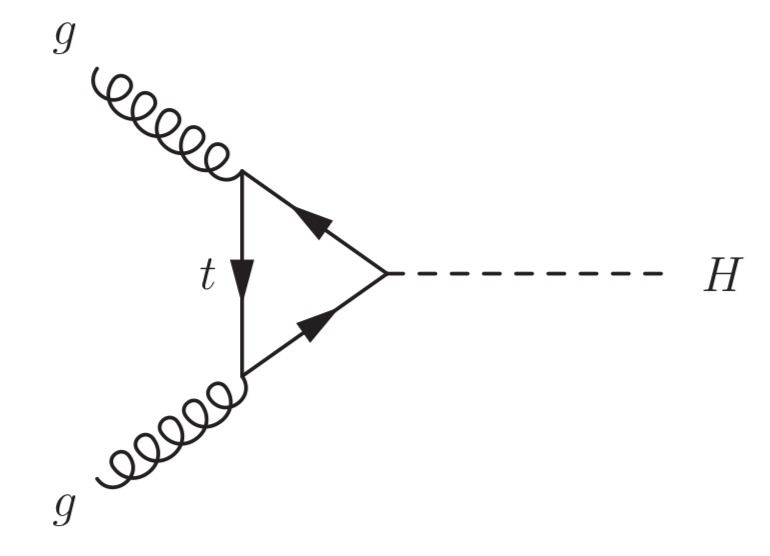
\includegraphics[width=0.8\textwidth]{figures/theory/ggF}
    \caption{$\ggf$}
  \end{subfigure}%
  \begin{subfigure}[b]{0.5\textwidth}
    \centering
    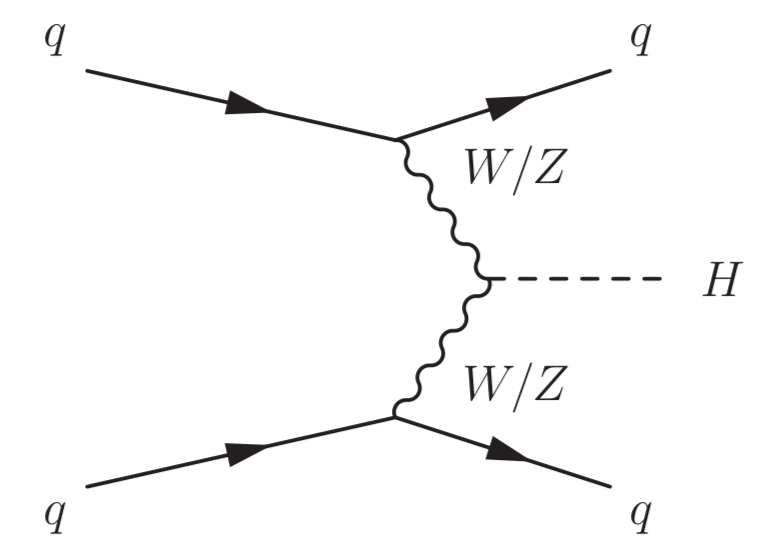
\includegraphics[width=0.8\textwidth]{figures/theory/VBF}
    \caption{$\vbf$}
  \end{subfigure}
  \begin{subfigure}[b]{0.5\textwidth}
    \centering
    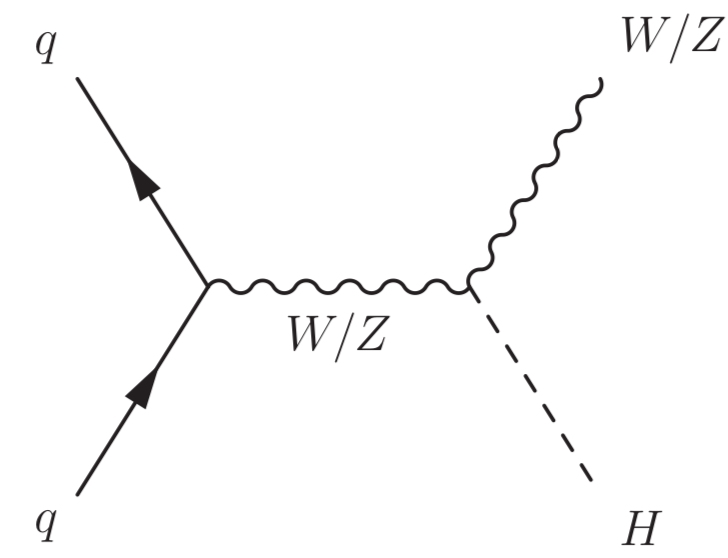
\includegraphics[width=0.8\textwidth]{figures/theory/VH}
    \caption{$\vh$}
  \end{subfigure}%
  \begin{subfigure}[b]{0.5\textwidth}
    \centering
    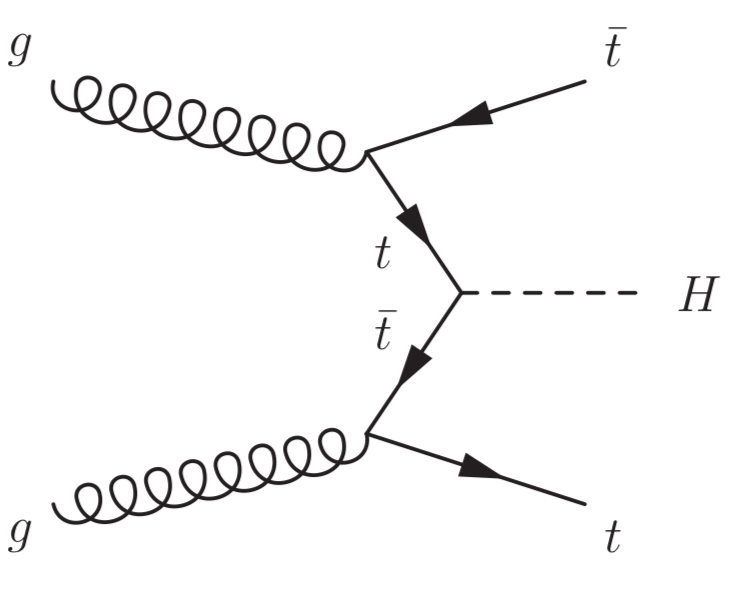
\includegraphics[width=0.8\textwidth]{figures/theory/ttH}
    \caption{$\tth$}
  \end{subfigure}
  \caption[Feynman diagrams for the four main Higgs boson production modes at the LHC.]
  {Feynman diagrams for the four main Higgs boson production modes at the LHC.
  $\ggf$ process is shown in the top left, $\vbf$ in the top right, $\vh$ in bottom left, and
  $\tth$ in the bottom right subfigure.}
   \label{fig:the:prod}
\end{figure}

The majority of the Higgs bosons at the LHC are produced via the $\ggf$ production mode,
followed by $\vbf$, $\vh$, and $\tth$ production. Another two production modes are $\bbh$
and $\tH$, but they are more difficult to tag experimentally. The cross-sections and
relative fractions depend on the centre-of-mass energy as shown in Figure \ref{fig:the:prod}.
At 13 \TeV, the production cross section for the $\ggf$ production mode is
$\sigma_{\ggf} = 48.58~\pb
~^{+4.56\%}_{-6.72\%}~(\text{theory})
\pm 3.20\%~(\text{PDF}+\alpha_S)$,
where the PDF stands for parton distribution functions and $\alpha_S$ refers to the strong
coupling constant. The total cross-section for the $\vbf$ production mode is
$\sigma_{\vbf} = 3781.7~\fb
~^{+0.43\%}_{-0.33\%}~(\text{scale})
\pm 2.1\%~(\text{PDF}+\alpha_S) $

\begin{figure}[h]
  \centering
  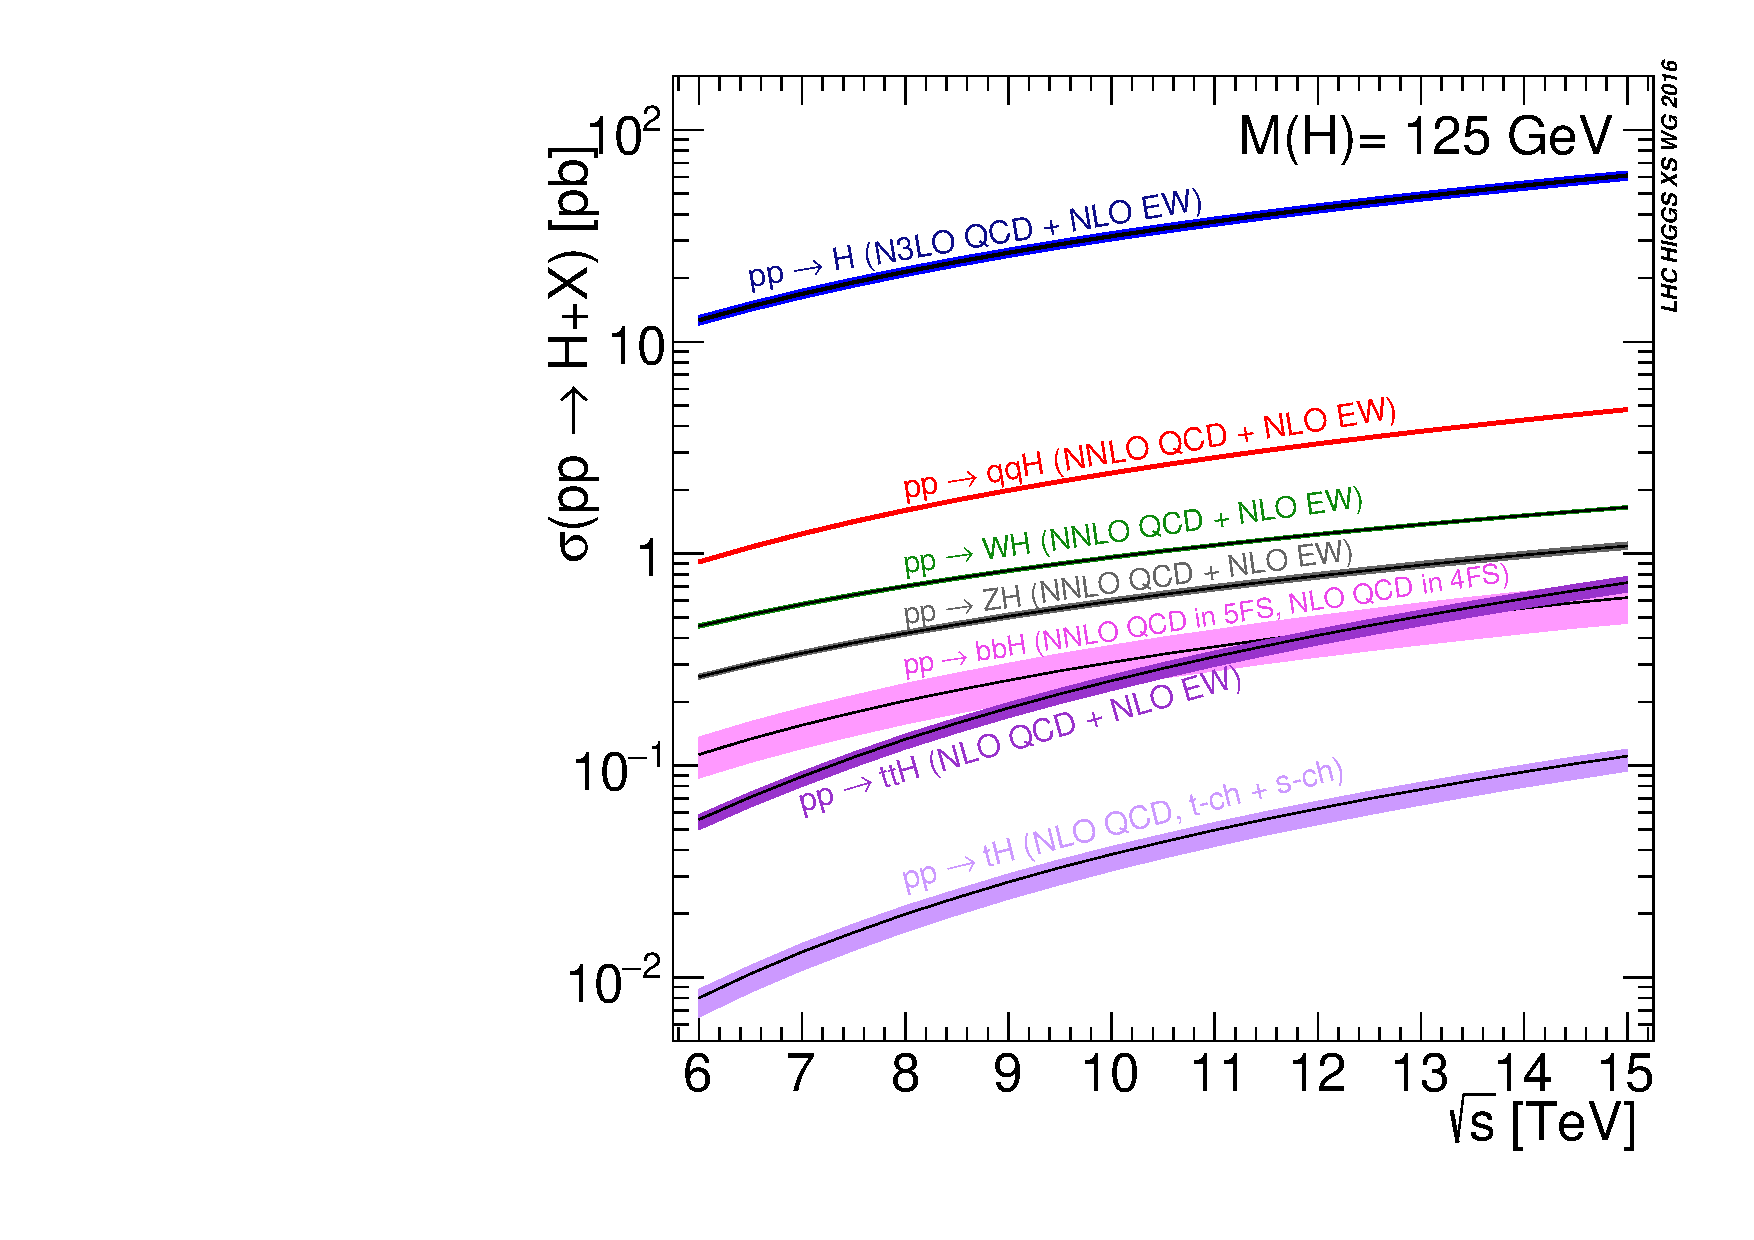
\includegraphics[width=0.8\textwidth]{figures/theory/HiggsProduction}
  \caption[Higgs boson production cross-sections at the LHC.]{Higgs boson production
  cross-sections at the LHC as a function of centre-of-mass energy, for a Higgs boson
  of mass $m_H = 125 \GeV$. $\ggf$ production cross section is shown in blue
  ($pp \rightarrow H$), $\vbf$ in red ($pp \rightarrow qqH$), and $\tth$ in purple
  ($pp \rightarrow ttH$), while $\vh$ is shown separately for the $W$ and $Z$ bosons
  in green and gray, respectively. From Ref. \cite{deFlorian:2016spz}.}
   \label{fig:the:prod}
\end{figure}

The Higgs boson is an unstable particle and can decay in a variety of ways. As noted,
the strength of the interaction with bosons and fermions is proportional to the mass,
meaning that the Higgs boson preferentially decays to the heavier particles, if they
are kinematically allowed. Figure \ref{fig:the:decay} shows the Higgs boson branching
ratios, defined as the fractions of the rate of a particular decay to the total
rate of decay. For the SM Higgs boson with $m_H = 125~\GeV$, the predicted decay rate to muon pairs
is $2.176 \times 10^{-4}
\pm 1.23\%~(\text{theory})
\pm 0.99\%~(\text{quark mass})
\pm 0.64\%~(\alpha_S)$ \cite{deFlorian:2016spz}. 

\begin{figure}[h]
  \centering
  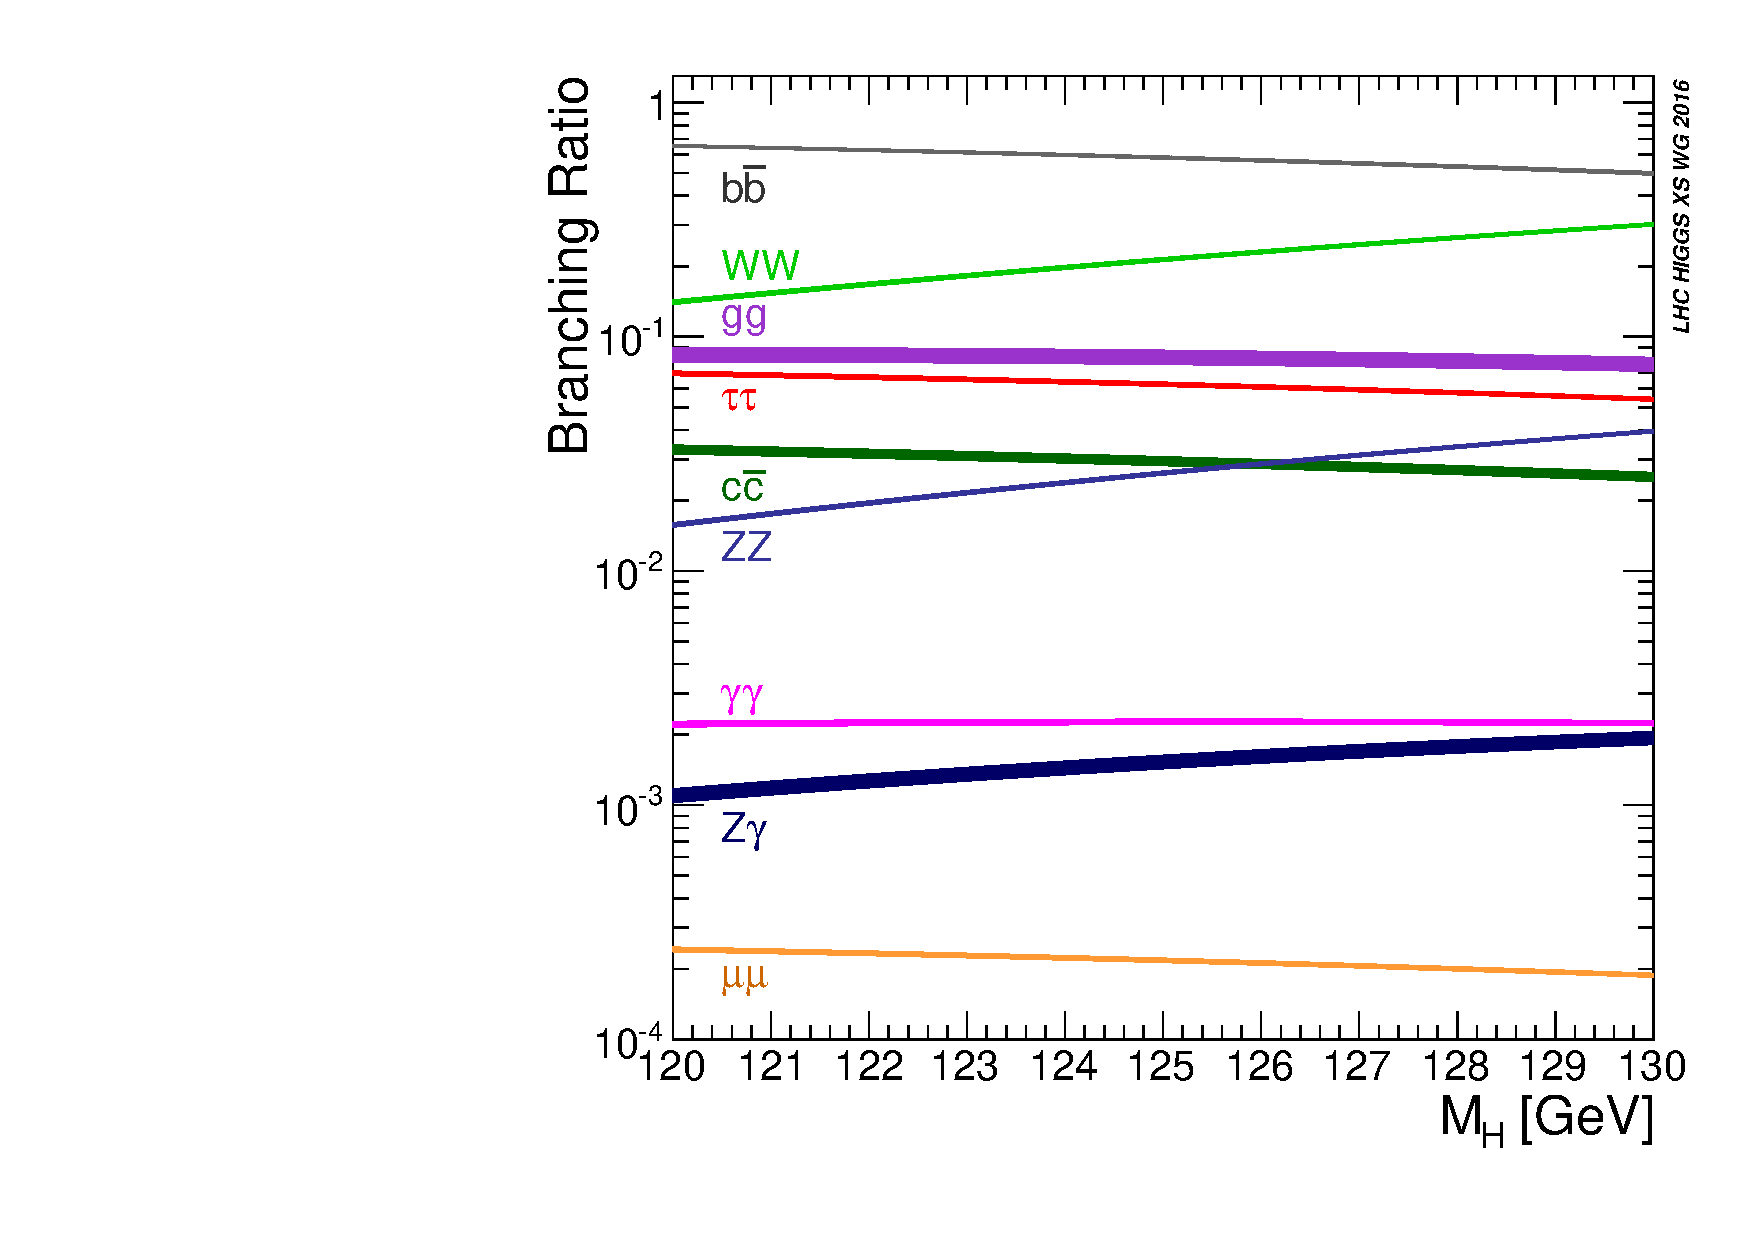
\includegraphics[width=0.8\textwidth]{figures/theory/HiggsDecay}
  \caption[Higgs boson branching ratios.]{Higgs boson branching ratios as a function
  of the Higgs boson mass. Branching ratio to muon pairs is shown in orange.
  From Ref. \cite{deFlorian:2016spz}.}
   \label{fig:the:decay}
\end{figure}

\section{Shortcomings}

The success
of the predictive power of the Standard Model is unparalleled in the history of science.
It has been tested to unprecedented levels of numerical precision and even predicted new
fundamental particles before any experimental evidence for their existence. However,
despite its successes, the SM has numerous shortcomings.

Experimentally, while it makes exceptionally
precise predictions on a vast number of the results of measurements over many orders
of magnitude, there are a few observations that it is unable to explain at all.
Cosmological observations have firmly established the existence of dark matter via its
gravitational interactions, and the existence of dark energy via the measurements of
the cosmic microwave background spectrum, none of which can be explained by the SM.
Similarly, the SM is unable to explain the matter-antimatter asymmetry in the universe.

From the theoretical perspective it is unsatisfactory that there is no quantum field description of gravity
in the SM. Additionally, the bare mass of the Higgs boson is considered to be
unnaturally close to its quantum corrections.

All of these shortcomings suggest that the SM is not a complete description of Nature.
Two complementary experimental strategies to search for physics beyond the SM are
employed at the LHC. The first approach directly searches
for yet unobserved phenomena that would reveal new particles. The second approach tests
the predictions of the SM in search for a discrepancy which would signal the direction
in which direct searches should be made. While the results of direct approaches are
more easily interpretable, the advantage of indirect approaches is that they can probe
particles kinematically inaccessible at the LHC. This thesis utilises the second
approach via the search for the decay of the Higgs boson to a muon pair. Any
statistically significant discrepancy between the measured and theoretically predicted
values would hint at the existence of new physics.

